\documentclass[11pt,twoside]{article}
\usepackage{geometry}
\usepackage{enumerate}
\usepackage{latexsym,booktabs}
\usepackage{amsmath,amssymb}
\usepackage{graphicx}
\usepackage{hyperref}
\usepackage[singlespacing]{setspace}
\usepackage{calc}
\usepackage{blindtext}
\usepackage{subfig}
\usepackage{graphicx}
\usepackage{tikz}
\usetikzlibrary{positioning}

\geometry{a4paper,left=2cm,right=2.0cm, top=2cm, bottom=2.0cm}

\newtheorem{Definition}{Definition}
\newtheorem{Theorem}{Theorem}
\newtheorem{Lemma}{Lemma}
\newtheorem{Corollary}{Corollary}
\newtheorem{Proposition}{Proposition}
\newtheorem{Algorithm}{Algorithm}
\numberwithin{Theorem}{section}
\numberwithin{Definition}{section}
\numberwithin{Lemma}{section}
\numberwithin{Algorithm}{section}
\numberwithin{equation}{section}

\newcommand{\dottedline}[1]{\makebox[#1]{.\dotfill}}

\begin{document}

\pagestyle{empty}

% =============================================================================
% Title page
% =============================================================================
\begin{titlepage}
\vspace*{.5em}
\center
\textbf{\Large{The School of Mathematics}} \\
\vspace*{1em}
\begin{figure}[!h]
\centering

\includegraphics[width=180pt]{CentredLogoCMYK.jpg}
\end{figure}
\vspace{2em}
\textbf{\Huge{Finding diferentially expressed genes in Cryptococcus neoformans across different design conditions}}\\[2em]
\textbf{\LARGE{by}}\\
\vspace{2em}
\textbf{\LARGE{Theodoros Ladas}}\\
\vspace{6.5em}
\Large{Dissertation Presented for the Degree of\\
MSc in Statistics with Data Science}\\
\vspace{6.5em}
\Large{July 2021}\\
\vspace{3em}
\Large{Supervised by\\Natalia Bochkina and Simon Taylor}
\vfill
\end{titlepage}

\cleardoublepage

% =============================================================================
% Executive summary, acknowledgments, and own work declaration
% =============================================================================
\begin{center}
\Large{Executive Summary}
\end{center}

In this dissertation project, data from a lab experiment of the University of Edinburgh on the fungus \emph{Cryptococcus neoformans} are being analyzed. More specifically, the fungus is cultivated in two different media, one nutrient-rich and one nutrient-poor, at two different temperatures. The goals of the analysis are first to find differentially expressed genes in the fungus' genome, and second to understand what are the k-mers that have high predictive power in predicting gene expression. The first goal was achieved by using various statistical tests to find statistically significant gene expression differences between conditions, while for the second task, four different machine learning methods were used to reach a robust conclusion.

\clearpage

\begin{center}
\Large{University of Edinburgh – Own Work Declaration}
\end{center}


This sheet must be filled in, signed and dated - your work will not be marked unless this is done.
\vspace{1cm}

Name: \dottedline{8cm}

Matriculation Number: \dottedline{6cm}

Title of work: \dottedline{8cm}

\vspace{1cm}

I confirm that all this work is my own except where indicated, and that I have:
\begin{itemize}
\item	Clearly referenced/listed all sources as appropriate	 				
\item	Referenced and put in inverted commas all quoted text (from books, web, etc)	
\item	Given the sources of all pictures, data etc. that are not my own				
\item	Not made any use of the report(s) or essay(s) of any other student(s) either past 	
or present	
\item	Not sought or used the help of any external professional academic agencies for the work
\item	Acknowledged in appropriate places any help that I have received from others	(e.g. fellow students, technicians, statisticians, external sources)
\item	Complied with any other plagiarism criteria specified in the Course handbook
\end{itemize}

I understand that any false claim for this work will be penalised in accordance with
the University regulations	(\url{https://teaching.maths.ed.ac.uk/main/msc-students/msc-programmes/statistics/data-science/assessment/academic-misconduct}).								

\vspace{1cm}

Signature \dottedline{8cm}

\vspace{5mm}

Date \dottedline{8cm}


\clearpage



% =============================================================================
% Table of contents, tables, and pictures (if applicable)
% =============================================================================
\pagestyle{plain}
\setcounter{page}{1}
\pagenumbering{Roman}

\tableofcontents
\clearpage
%\listoftables
\listoffigures
\cleardoublepage

\pagenumbering{arabic}
\setcounter{page}{1}

\nocite{*}
\clearpage

% ------------------------------------------------------------------------------------------------------
\section{Introduction}
\subsection{Motivation}
\label{sec:motivation}

Cryptococcosis identified in 1894 is an invasive fungal infection that presents substantial therapeutic challenges. It is caused by species within the genus Cryptococcus which is divided into two subspecies, \emph{C. gattii} and \emph{C. neoformans}. Cryptococcus invades the human lungs, where it can cause pneumonia in immunosuppressed patients. In immunocompetent hosts, the fungal cells are either cleared by the immune system or establish an asymptomatic latent infection \cite{may2016cryptococcus}. In the latter case, the fungi can potentially be a threat to their host if the immune system is weakened for other reasons. 

In some environmental conditions, the fungi grow, which later results in Cryptococcosis manifesting symptoms. Thus, we can experimentally test in different conditions and across time what causes the fungus to grow or hide. In addition, in these experimental conditions, the genome of the virus can be studied to find what genes are expressed in these different conditions. This will enrich our understanding of the mechanism behind Cryptococcosis behaviour, thus resulting in potential treatments.

Each gene is made up of DNA, and DNA is a molecule of polynucleotide chains built by four bases adenine (A), thymine (T), cytosine (C), and guanine (G). In an effort to deepen our understanding of the mechanism of the fungus, after finding which genes are differentially expressed, we can also examine which motifs of these genes are important in predicting gene expression. The motifs of the genes are measured by counting how many k-mers can be found in each gene. An example of a k-mer where $k=4$ is \emph{AATG}. Since the gene can have a DNA chain that is thousands of bases long, it is important to use these k-mers to model the gene, as otherwise, the dataset could potentially become too large to work with consistently with traditional systems such as laptops or desktop computers. By isolating the genes that are differentially expressed, we can then perform various feature selection methods to test whether we can predict how much these genes are expressed from a few k-mers.

The way gene expression is measured is by RNA-sequencing. High throughput sequencing is a procedure in which we measure which genes in the chromosome are active and how much they are transcribed by measuring the messenger RNA transcription of the gene. This complex process involves preparing a sequence library, then sequencing the genes, and finally analysing the results. The scope of this dissertation project is to help with the last part (data analysis), as the dataset provided is already prepared and cleaned. The datasets provided are explained in detail in \autoref{sec:data}.  

\subsection{Experiment}
\label{sec:experiment}

The fungus was observed for 120 minutes by taking samples in 4-time points (10 minutes, 30 minutes, 60 minutes, and 120 minutes) in two different mediums (RPMI+serum, YPD) and at two different temperatures (25 C and 37 C). In addition to that, two biological replicates were tested. The difference in the media is that YPD is a nutrient-rich medium designed for yeast growth, while RPMI+serum is a nutrient-poor or host-like medium intended to mimic the human environment. 

It was observed that in both temperatures, in the RPMI+serum medium, the fungus developed a protective shell around it, while in the YPD medium, the cell grew. Thus, by measuring how much each gene is expressed in each of these conditions over time, we can understand what is causing the fungus to behave differently in these experimental conditions. 

\subsection{Dataset}
\label{sec:data}

Three different datasets were provided for exploration and analysis. 
\begin{itemize}
\item A file where the results of the estimated gene counts are measured across the various design conditions (medium, temperature, time, and biological replicate). Each row of the file represents a particular gene in a specific condition. The conditions are represented in the form of an encoded string; for example, "RC01A" means 
\begin{itemize}
\item Medium: R (RPMI+serum)
\item Temperature: C (25 C)
\item Time: 01 (10 minutes)
\item Replicate: A

\end{itemize}
\item A metafile, where all the explanations for the different conditions are logged.
\item A file containing the k-mers with $k=4$ for all the genes found in the chromosomes of \emph{C. neoformans}.
\end{itemize}

\subsection{Technologies}
\label{sec:technologies}

For the purposes of this analysis, the \textsf{R} language was used to load and analyse the dataset. In addition to that, the \textsf{DESeq2} library \cite{love2014moderated} was used to find the differentially expressed genes. This library is used to analyse read counts per gene in RNA-seq in order to discover whether systemic changes in gene expression exist across experimental conditions. The analysis is run in a \textsf{Linux} based system, with 16GB of RAM. 

\clearpage
%------------------------------------------------------------------------------------------------------
\section{Exploratory Data Analysis}
\label{sec:eda}

In this section, various exploratory graphs and other figures are provided in order to understand what is useful for the research questions and what is not. These consist of a univariate and bivariate analysis, as well as the unsupervised machine learning technique of Principal Component Analysis (PCA). The univariate analysis is essential because it reveals the distribution of the target variable, the gene expression. The bivariate analysis is used in order to find a potential correlation between features, and lastly, PCA will reveal which combinations of features are predictive or not.

\subsection{Univariate Analysis}
\label{sec:univariate}

By plotting the estimated counts, alongside the transcripts per million and the fold change variables, we see in \autoref{fig:uni} (a) that they all contain the same level of information. This is because the distribution of the target variable is highly skewed to the right, with the majority of its mass around zero. 

% \begin{figure}[h]
%     \centering
%     \subfloat[Correlation matrix]
%     {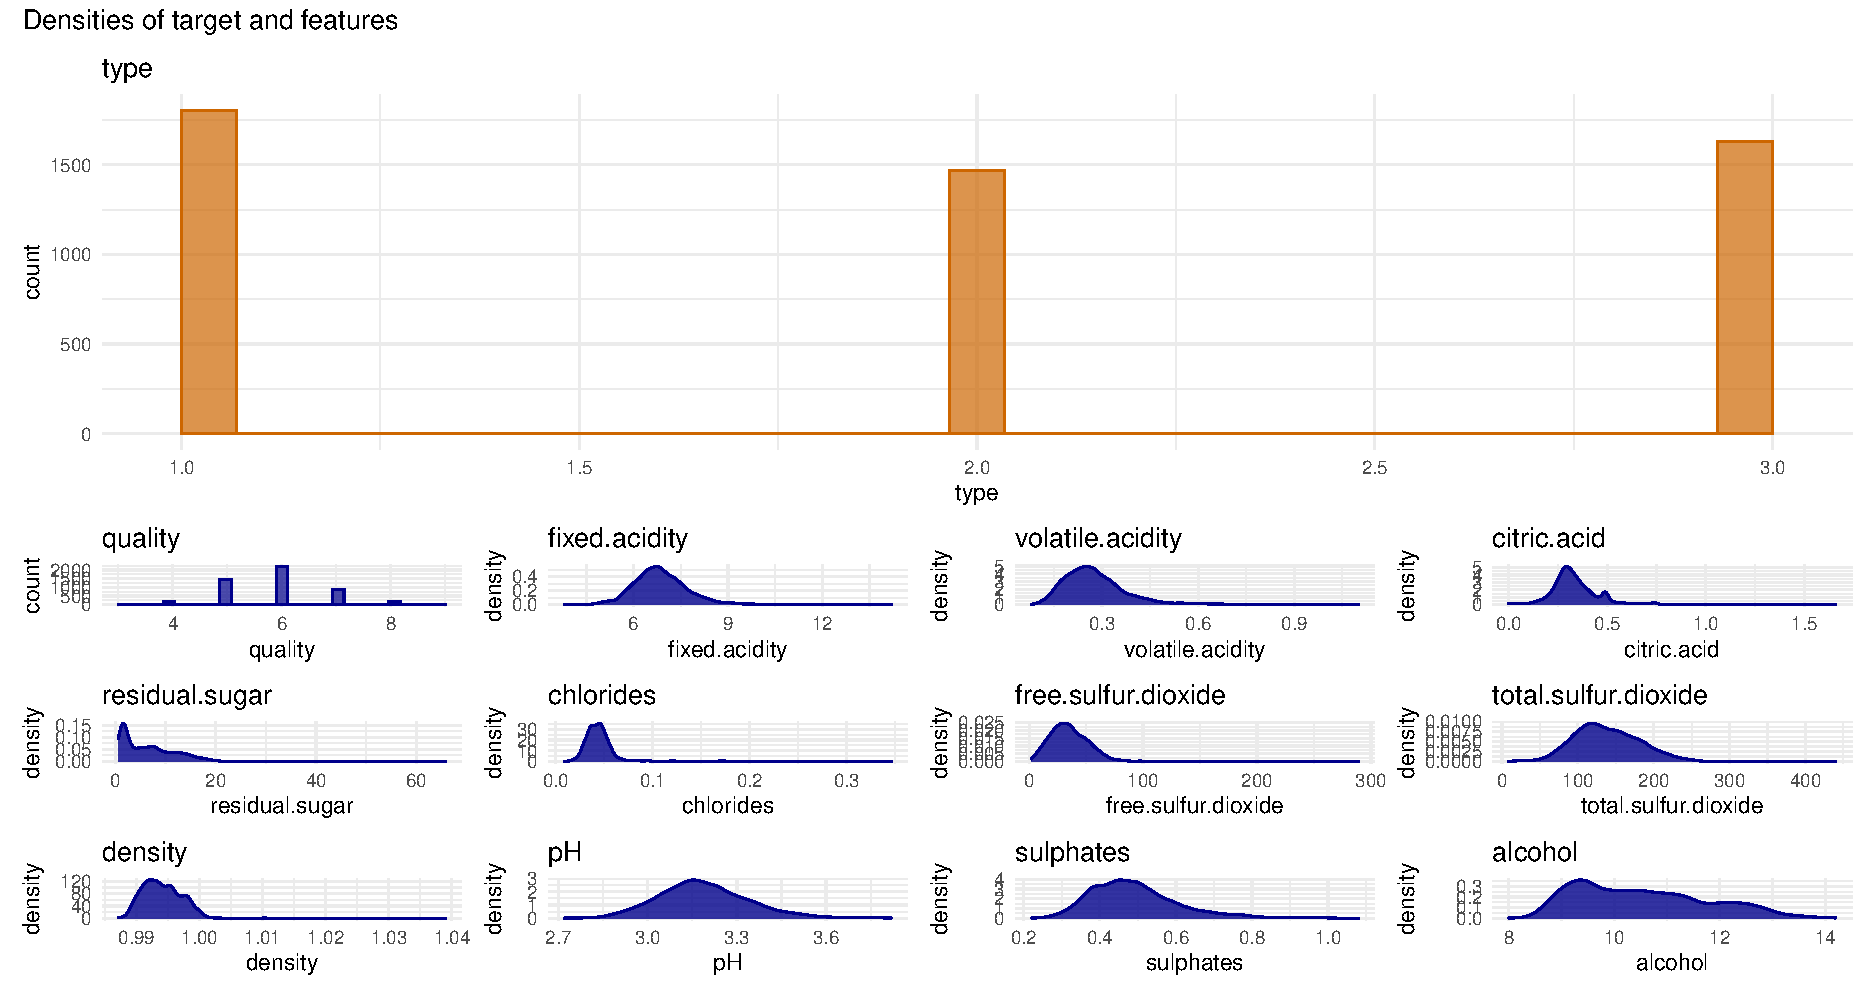
\includegraphics[width=.4\textwidth,height=.25\textheight]{./output/1.e.corrplot-1.pdf}}
%     \subfloat[Correlation network]
%     {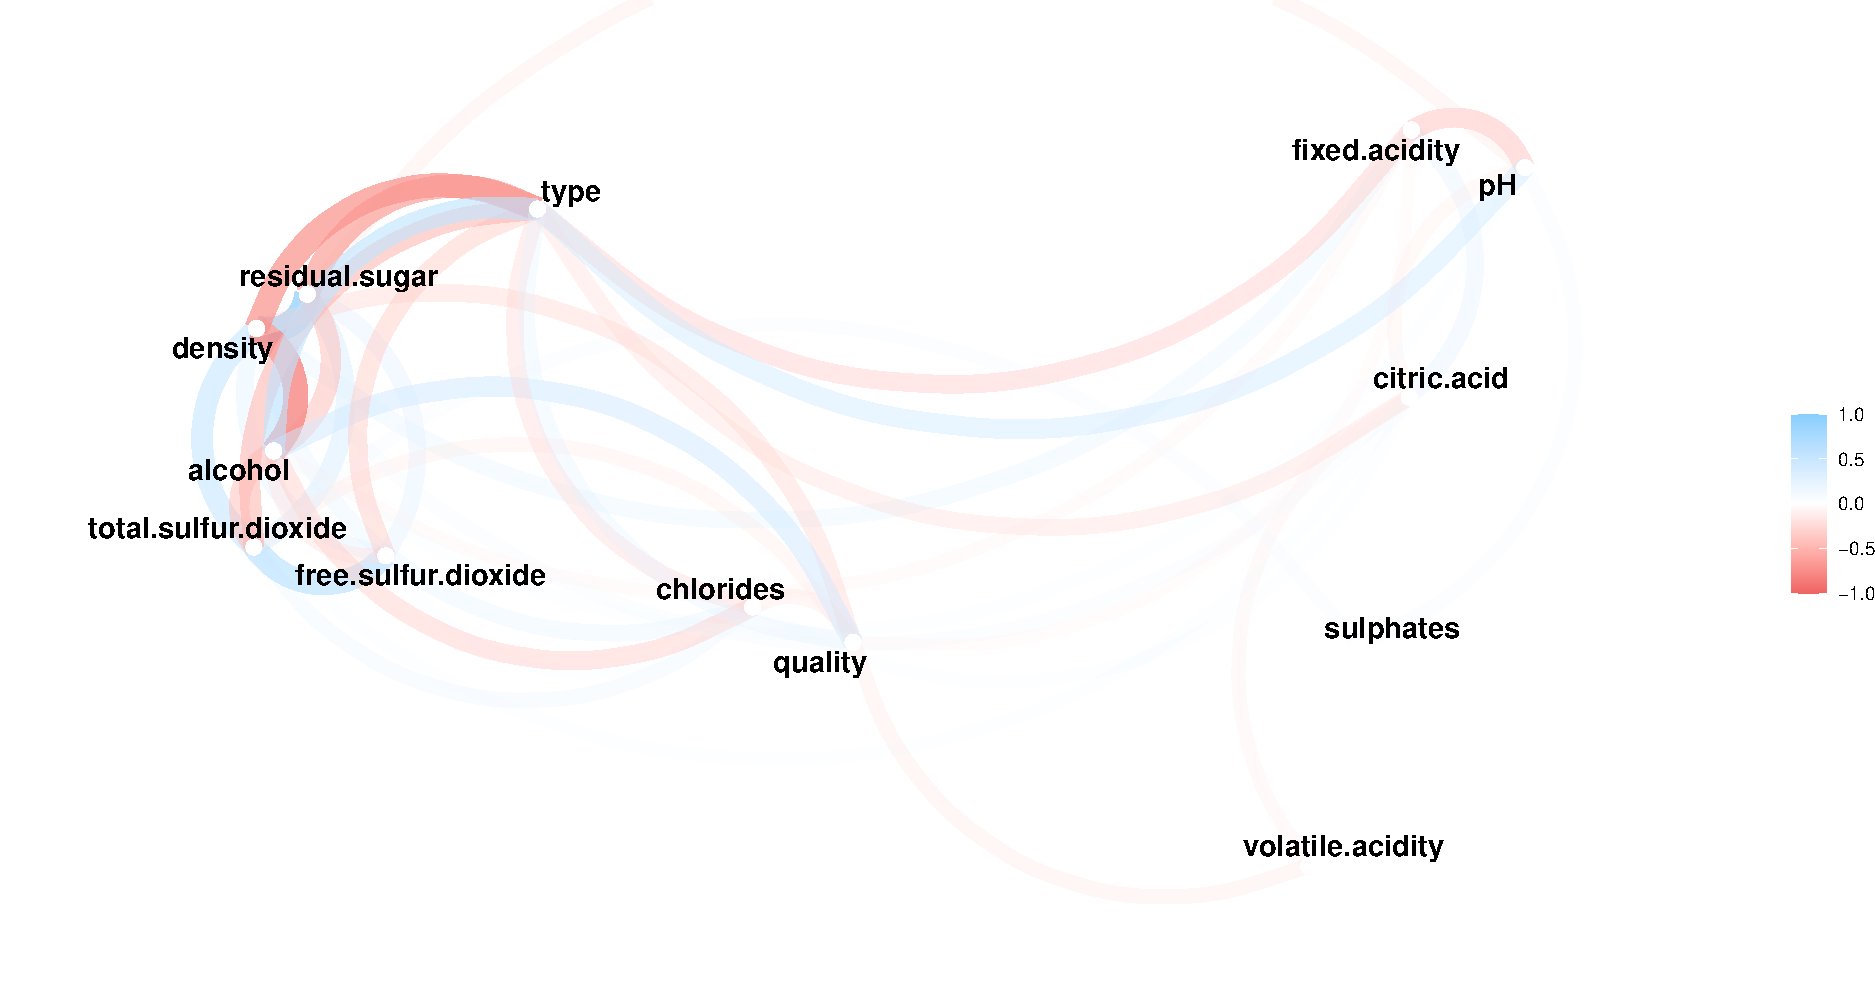
\includegraphics[width=.6\textwidth]{./output/1.f.corplot-2.pdf}}
%     \caption{Bivariate EDA of Dataset}
%     \label{fig:corr}
% \end{figure}

\begin{figure}[h]
    \centering
    \subfloat[Distribution of gene expression variables]
    {\includegraphics[width=.5\textwidth]{./output/univariate-analysis.pdf}}
    \subfloat[Estimated Counts accross media]
    {\includegraphics[width=.5\textwidth]{./output/est_counts_per_medium.pdf}}
    \caption{Univariate Analysis Results}
    \label{fig:uni}
\end{figure}

This shape could be modelled by a lognormal distribution, even though it is not an exact fit. Since the variable "estimated counts" is the simplest one of the others, the analysis is going to take place with this as the target variable. 

We can take a closer look at the estimated counts' distribution by plotting it between conditions to see if there exists any change. For example, in \autoref{fig:uni} (b), we see that the distribution is practically the same between the two media. That means that our different classes are balanced between the two media. In \autoref{sec:pca} a more robust way of looking at imbalances will be presented. 

\subsection{Bivariate Analysis}
\label{sec:bivariate}

In \autoref{fig:biv} a confusion matrix that measures the correlation between variables is presented, which extends the univariate analysis. For measuring the correlation, the \textit{Pearson's correlation coefficient} is used. This coefficient measures the covariance of two random variables, $X$ and $Y$, after normalising it with the product of their standard deviations by \autoref{eqn:corr}.

\begin{equation}
\label{eqn:corr}
\rho(x,y) = \frac{\text{cov}(x,y)}{\text{std}(x)\text{std}(y)}
\end{equation}


\vspace*{1em}
\begin{figure}[]
\centering
\includegraphics[width=0.7\textwidth]{./output/bivariate-analysis.pdf}
\caption{Confusion Matrix}
\label{fig:biv}
\end{figure}
\vspace{2em}

The expected finding, as observed on the bottom right corner of \autoref{fig:biv}, is that the estimated counts and the transcripts per million are highly correlated. This is expected, as TPM is a normalised version of the estimated counts. However, a more important finding is the fact that some k-mers are highly correlated with each other. The k-mers that are related to each other also have the same bases but in a different order (for example, \emph{aata}, and \emph{ataa}). This is something that needs further explanation, as it happens in around $12$ pairs of k-mers out of the $130$ possible pairs. 

\subsection{PCA}
\label{sec:pca}

In an attempt to better understand the sources of variation in the condition, the unsupervised machine learning technique of Principal Components Analysis was implemented. The dataset that was used to create this plot was one with the estimated counts and a one-hot-encoded version of the conditions.

\begin{figure}[h]
    \centering
    \subfloat[Cumalative variance explained]
    {\includegraphics[width=.5\textwidth]{./output/variance-expl.pdf}}
    \subfloat[Feature importance of first four Principal Components]
    {\includegraphics[width=.5\textwidth]{./output/first-pcs-explaines.pdf}}
    \caption{Principal Component Analysis results}
    \label{fig:pca}
\end{figure}

In \autoref{fig:pca} (a), it is clear that with just the first four principal components, we can explain almost all the variation in the dataset. Therefore in \autoref{fig:pca} (b), a more in-depth analysis of what those first four principal components are is presented. 

We see that the most significant source of variation can be explained by looking at which medium the fungus has been transferred. This is expected as the media in which the fungi are cultivated is one of the most critical aspects of the experiments. However, the second most significant variation factor is whether the measurement taken belongs to biological replicate A or B. This is surprising and should not be observed, as the reason for taking multiple replicates is to build confidence in the statistical methods used and not to use it as a predictor for the target variable. In \autoref{sec:bias}, more details on how this bias was corrected will be presented. Lastly, the third and the fourth principal components show that the temperature, the second most crucial factor in the experiment, is a significant source of variance in the dataset. It even prioritises the 25 C vs 37 C before the 30 C vs 37 C temperature difference.

In summary, the principal components analysis gave us valuable insights. First, it identified that there exists a variation within the data, and it is affected firstly by the medium in which the fungi were cultivated and secondly by the temperature difference, which is an important finding to continue with the research. However, it also revealed the existence of a bias in the dataset between the two biological replicates that needs to be corrected before trying to find differentially expressed genes.

\subsection{Bias correction}
\label{sec:bias}

Before moving to methods to identify differentially expressed genes, the bias between biological replicates, A and B, need to be accounted for. In order to deal with this, a smooth splines regression method is used. The reason this method is used is due to the flexibility of the technique to capture non-linearities in the data. A spline is a special case of polynomial regression \cite{ridgeway2007all}. The dataset is split into various sections, marked by knots, and a polynomial regression line is fitted in each section. The restriction of the splines method is that at the knots, the function must be continuous and twice differentiable to ensure that it is smooth. 

\vspace*{1em}
\begin{figure}[]
\centering
\includegraphics[width=0.7\textwidth]{./output/bias-correction.pdf}
\caption{Smooth splines difference}
\label{fig:splines}
\end{figure}
\vspace{2em}

Let $y_1$ be the estimated counts of biological replicate A, and $y_2$ be the estimated counts of biological replicate B. In \autoref{fig:splines} we see that the difference of the two in the $y$ axis. If no bias were observed, the difference would be zero for every value of $y_2$; the red line is the smooth spline regression fit of $y_1$ and $y_2$, with a lambda coefficient of $\lambda = 0.01$. 

This represents the bias in the two vectors (positive or negative). Therefore we can correct $y_1$ by adding the result in the original vector ($y' = y + bias$). 

\clearpage
% ------------------------------------------------------------------------------------------------------
\section{Differentially Expressed Genes}
\label{sec:diff}

After the exploratory data analysis and the bias correction, we looked into methods to find differentially expressed genes. However, before searching for those in a consistent way, some simple plots will show whether we should expect to see these differentially expressed genes or not. For example, in \autoref{fig:mostleast}, the five genes with the most (least) overall change in estimated counts are plotted in a time-series plot. The overall change is calculated by simply taking the percent change over the $t=0$ and $t=120$. This shows us that we expect to find some genes that are expressed more than others by condition. 

\vspace*{1em}
\begin{figure}[!h]
\centering
\includegraphics[width=0.7\textwidth]{./output/most-vs-least.pdf}
\caption{Top 5 Most and Least expressed genes accross conditions over time}
\label{fig:mostleast}
\end{figure}
\vspace{2em}

This can also be verified by \autoref{fig:mostleast-conditions}. Thus, for example, the condition with ID, YW18B which represents, the YPD medium, at 37 C, on the 180 minutes, of biological replicate B has around 3 million total estimated counts, while condition YH12B has less than half a million. 

\vspace*{1em}
\begin{figure}[!h]
\centering
\includegraphics[width=0.7\textwidth]{./output/most-vs-least-conditions.pdf}
\caption{Sum of estimated counts for all possible conditions}
\label{fig:mostleast-conditions}
\end{figure}

This means that it is expected to find differentially expressed genes by running various statistical tests.

\subsection{Statistical Tests}
\label{tests}

In order to conclude which genes are differentially expressed, a statistical t-test in each condition (temperature and medium) was conducted with the two replicates as our sample values in order to determine whether the gene was expressed or not. The t-test is a statistical test based on the Student t distribution. For the test across media, the null hypothesis is that the mean estimated counts between media (YPD and RPMI+) are statistically the same. Hence, the interpretation of the p-value produced by the test for each gene can be thought of as the probability that the observed change in estimated counts happened by chance and not due to the difference in media. A p-value of less than $5\%$ is a typical threshold because it means that there is a $95\%$ chance for the result to be due to the media change \emph{ceteris paribus}, than chance. 

\begin{figure}[h]
    \centering
    \subfloat[p-values adjusted between Temperatures]
    {\includegraphics[width=.5\textwidth]{./output/volcano-temp.pdf}}
    \subfloat[p-values adjusted between Media]
    {\includegraphics[width=.5\textwidth]{./output/volcano-medium.pdf}}
    \caption{Volcano plots of p-values}
    \label{fig:volcano}
\end{figure}

In \autoref{fig:volcano} the volcano plots for the two tests, one on medium and the other on temperatures, are shown. \autoref{fig:volcano} (a) is showing the p-values in a log-transformed scale, while \autoref{fig:volcano} (b) shows the unscaled version. The dots pointed in red are the genes, the p-values of which are less than the set threshold of $5\%$.  Therefore, by taking into consideration the intercept of these two tests, a conclusion can be reached for the genes that are differentially expressed both in temperature and media. Information regarding additional methods and caveats can be found on \autoref{sec:discussion}.

\vspace*{1em}
\begin{figure}[!h]
\centering
\includegraphics[width=0.7\textwidth]{./output/most-expressed-gene.pdf}
\caption{Most expressed gene across both conditions}
\label{fig:topgene}
\end{figure}
\vspace{2em}

In \autoref{fig:topgene}, the most expressed gene with a p-value less than $0.05$ is presented. The normalised count is the logarithm base two of the fold change of the gene. It is clear from the graph that on the RPMI+ medium, independently of the temperature, the gene "GNAG\_02060" is expressed more than in the YPD medium. This means that this method can produce some interpretable results.

\clearpage
% ------------------------------------------------------------------------------------------------------
\section{Informative Motifs}
\label{sec:diff}

The final goal of this dissertation project is to identify important k-mers on those genes that are informative of the gene expression. This is a feature selection task, as we need to identify a few k-mers, out of which we can build a model to predict which genes would be expressed. The motivation behind this step is that if a successful model is created, then the expensive steps of performing the experiment and the RNA sequencing could be avoided.

In order to find these features, multiple methods have been used to calculate feature importance. In the end, a voting system is implemented to find the intersection of the results. The models used had the estimated counts in a logarithmic transform as a target variable, as EDA showed that this could be the distribution of the estimated counts. The models used to provide the results were:
\begin{itemize}
\item A linear model with the full set of features as covariates
\item A Boruta model
\item A Lasso Model 
\item An sequential univariate linear model, where each feature is used as a covariate one by one
\end{itemize}

For the models that could potentially overfit, cross-validation was used to overcome this problem and ensure that the results are robust. In addition to that, these models were run on three different datasets. The first was the full dataset consisting of the logarithm of the estimated counts, the condition in a one-hot encoded version, and all the k-mers as features. In this dataset, each row represents a particular gene in some condition. The second was the subset of the full dataset, including only the genes that were differentially expressed, and the last one was the complementary of that or all the non-differentially expressed genes. 

\subsection{Full Linear Model}
\label{sec:full}

This is a simple linear model that minimises the sum of square errors in order to produce the Best Linear Unbiased Estimators (BLUE) as stated by the Gauss-Markov theorem \cite{eaton1983gauss}. Each coefficient of that model has an associated p-value. This p-value is used to answer the null hypothesis of the coefficient being precisely zero. Hence, by assuming that all the coefficients that have a p-value bigger than the threshold of $0.05$, we can eliminate those covariates as non-significant in predicting the gene expression. 

\subsection{Boruta Model}
\label{sec:boruta}

The Boruta algorithm is an iterative algorithm where each feature is iteratively tested against a shadow attribute \cite{kursa2010feature}. This shadow attribute is a randomised version of the actual feature. Hence, by comparing whether or not the actual features can perform better than the perturbed ones, we can conclude that some of these features are important while others are not. The experiment is the run for $500$ iterations for the three different datasets in order to build confidence intervals for the importance of each feature and conclude which features could be excluded. 

\subsection{LASSO Model}
\label{sec:lasso}

Consider the standard multivariate regression model where we predict $y_i$ at a linear function of $w_0$ and $N$ predictor variables. Consider choosing the coefficients $(w_1,w_2, ..., w_N)$ by minimising the sum of squared residuals plus a penalty term of the form:
\\
\begin{equation}
\lambda \sum_{i=1}^{N}[(1-\alpha)|w_i| + \alpha |w_i|^2]
\end{equation}
\\
If there is no penalty term $(\lambda = 0)$ this is ordinary least squares. If $(\alpha = 1)$ this is ridge regression and if $(\alpha = 0)$ this is called LASSO "least absolute shrinkage and selection operator". This penalised regression is a classic example of regularisation. In this case, the complexity is the number and size of the predictors in the model. All the above methods tend to shrink the coefficients towards zero. Hence it is a relatively straightforward way to do variable selection \cite{varian2014big}. The $\lambda$ parameter is called a hyperparameter of the model, and it was tuned by cross-validation. 

\subsection{Sequential univariate liner Model}
\label{sec:seq}

The last technique used to perform feature selection is a sequential univariate linear regression. It is the same as the first technique (Full Linear Model), but the features are used one by one instead of using all the covariates at once for prediction. This solves potential problems of multicollinearity. These models have a very high error. However, the reason they are selected is not for their power in prediction but for their straightforward interpretation of the coefficients of the covariates. 
\clearpage
% ------------------------------------------------------------------------------------------------------

\section{Results}
\label{sec:results}

In this section, the results of the important k-mers will be presented. The total table is included in the final files, as it is impossible to present more than $80$ k-mers in this report. However, a closer look is needed at the methods used to discover these results. The multivariate and univariate linear regression models do not need any explanation, as there is no overfitting possible in these kinds of models. 

However, the boruta and the Lasso models need a closer interpretation of their results. In \autoref{fig:lasso}, we see the mean square error for each value of the $\lambda$ hyperparameter. In addition, the confidence interval of the mean square error is also plotted in the form of error bars. The vertical dotted lines represent the $\lambda$ with the minimum mean square error as well as the one standard deviation $\lambda$. For the purposes of this experiment, the minimum was chosen; however, the results do not change significantly in the case the one standard deviation $\lambda$ is chosen. The integer numbers on the top of each diagram represent how many covariates have non-zero coefficients.

\begin{figure}[h]
    \centering
    \subfloat[Full model]
    {\includegraphics[width=.3\textwidth]{./output/lasso-full.pdf}}
    \subfloat[Only differentially expressed genes]
    {\includegraphics[width=.3\textwidth]{./output/lasso-diff.pdf}}
    \subfloat[All other genes]
    {\includegraphics[width=.3\textwidth]{./output/lasso-other.pdf}}
    \caption{Lasso model results}
    \label{fig:lasso}
\end{figure}

In all three diagrams, the same pattern emerges, as the best $\lambda$ value is around $1e-4$ (the logarithm is of the base $10$). For very low (numerically zero) values of $\lambda$, almost all $260$ variables have non-zero coefficients because as $\lambda$ tends to be zero, the LASSO model converges to the linear regression model. 

The boruta model is represented by the importance box plot in \autoref{fig:boruta}. In each diagram, the features are on the x-axis, while the importance score is on the y axis. The box plot can be drawn due to the iterative nature of the algorithm. Interestingly, almost all features are important in the subsection of the dataset where only differentially expressed genes are chosen.

\begin{figure}[h]
    \centering
    \subfloat[Full model]
    {\includegraphics[width=.3\textwidth]{./output/boruta-full.pdf}}
    \subfloat[Only differentially expressed genes]
    {\includegraphics[width=.3\textwidth]{./output/boruta-diff.pdf}}
    \subfloat[All other genes]
    {\includegraphics[width=.3\textwidth]{./output/boruta-other.pdf}}
    \caption{Boruta model results}
    \label{fig:boruta}
\end{figure}

After consolidating all the features in one data frame, we can count how many times the different methods selected each feature. In \autoref{fig:venn}, a Venn diagram of the various genes per dataset explored is presented. 

\vspace*{1em}
\begin{figure}[!h]
\centering
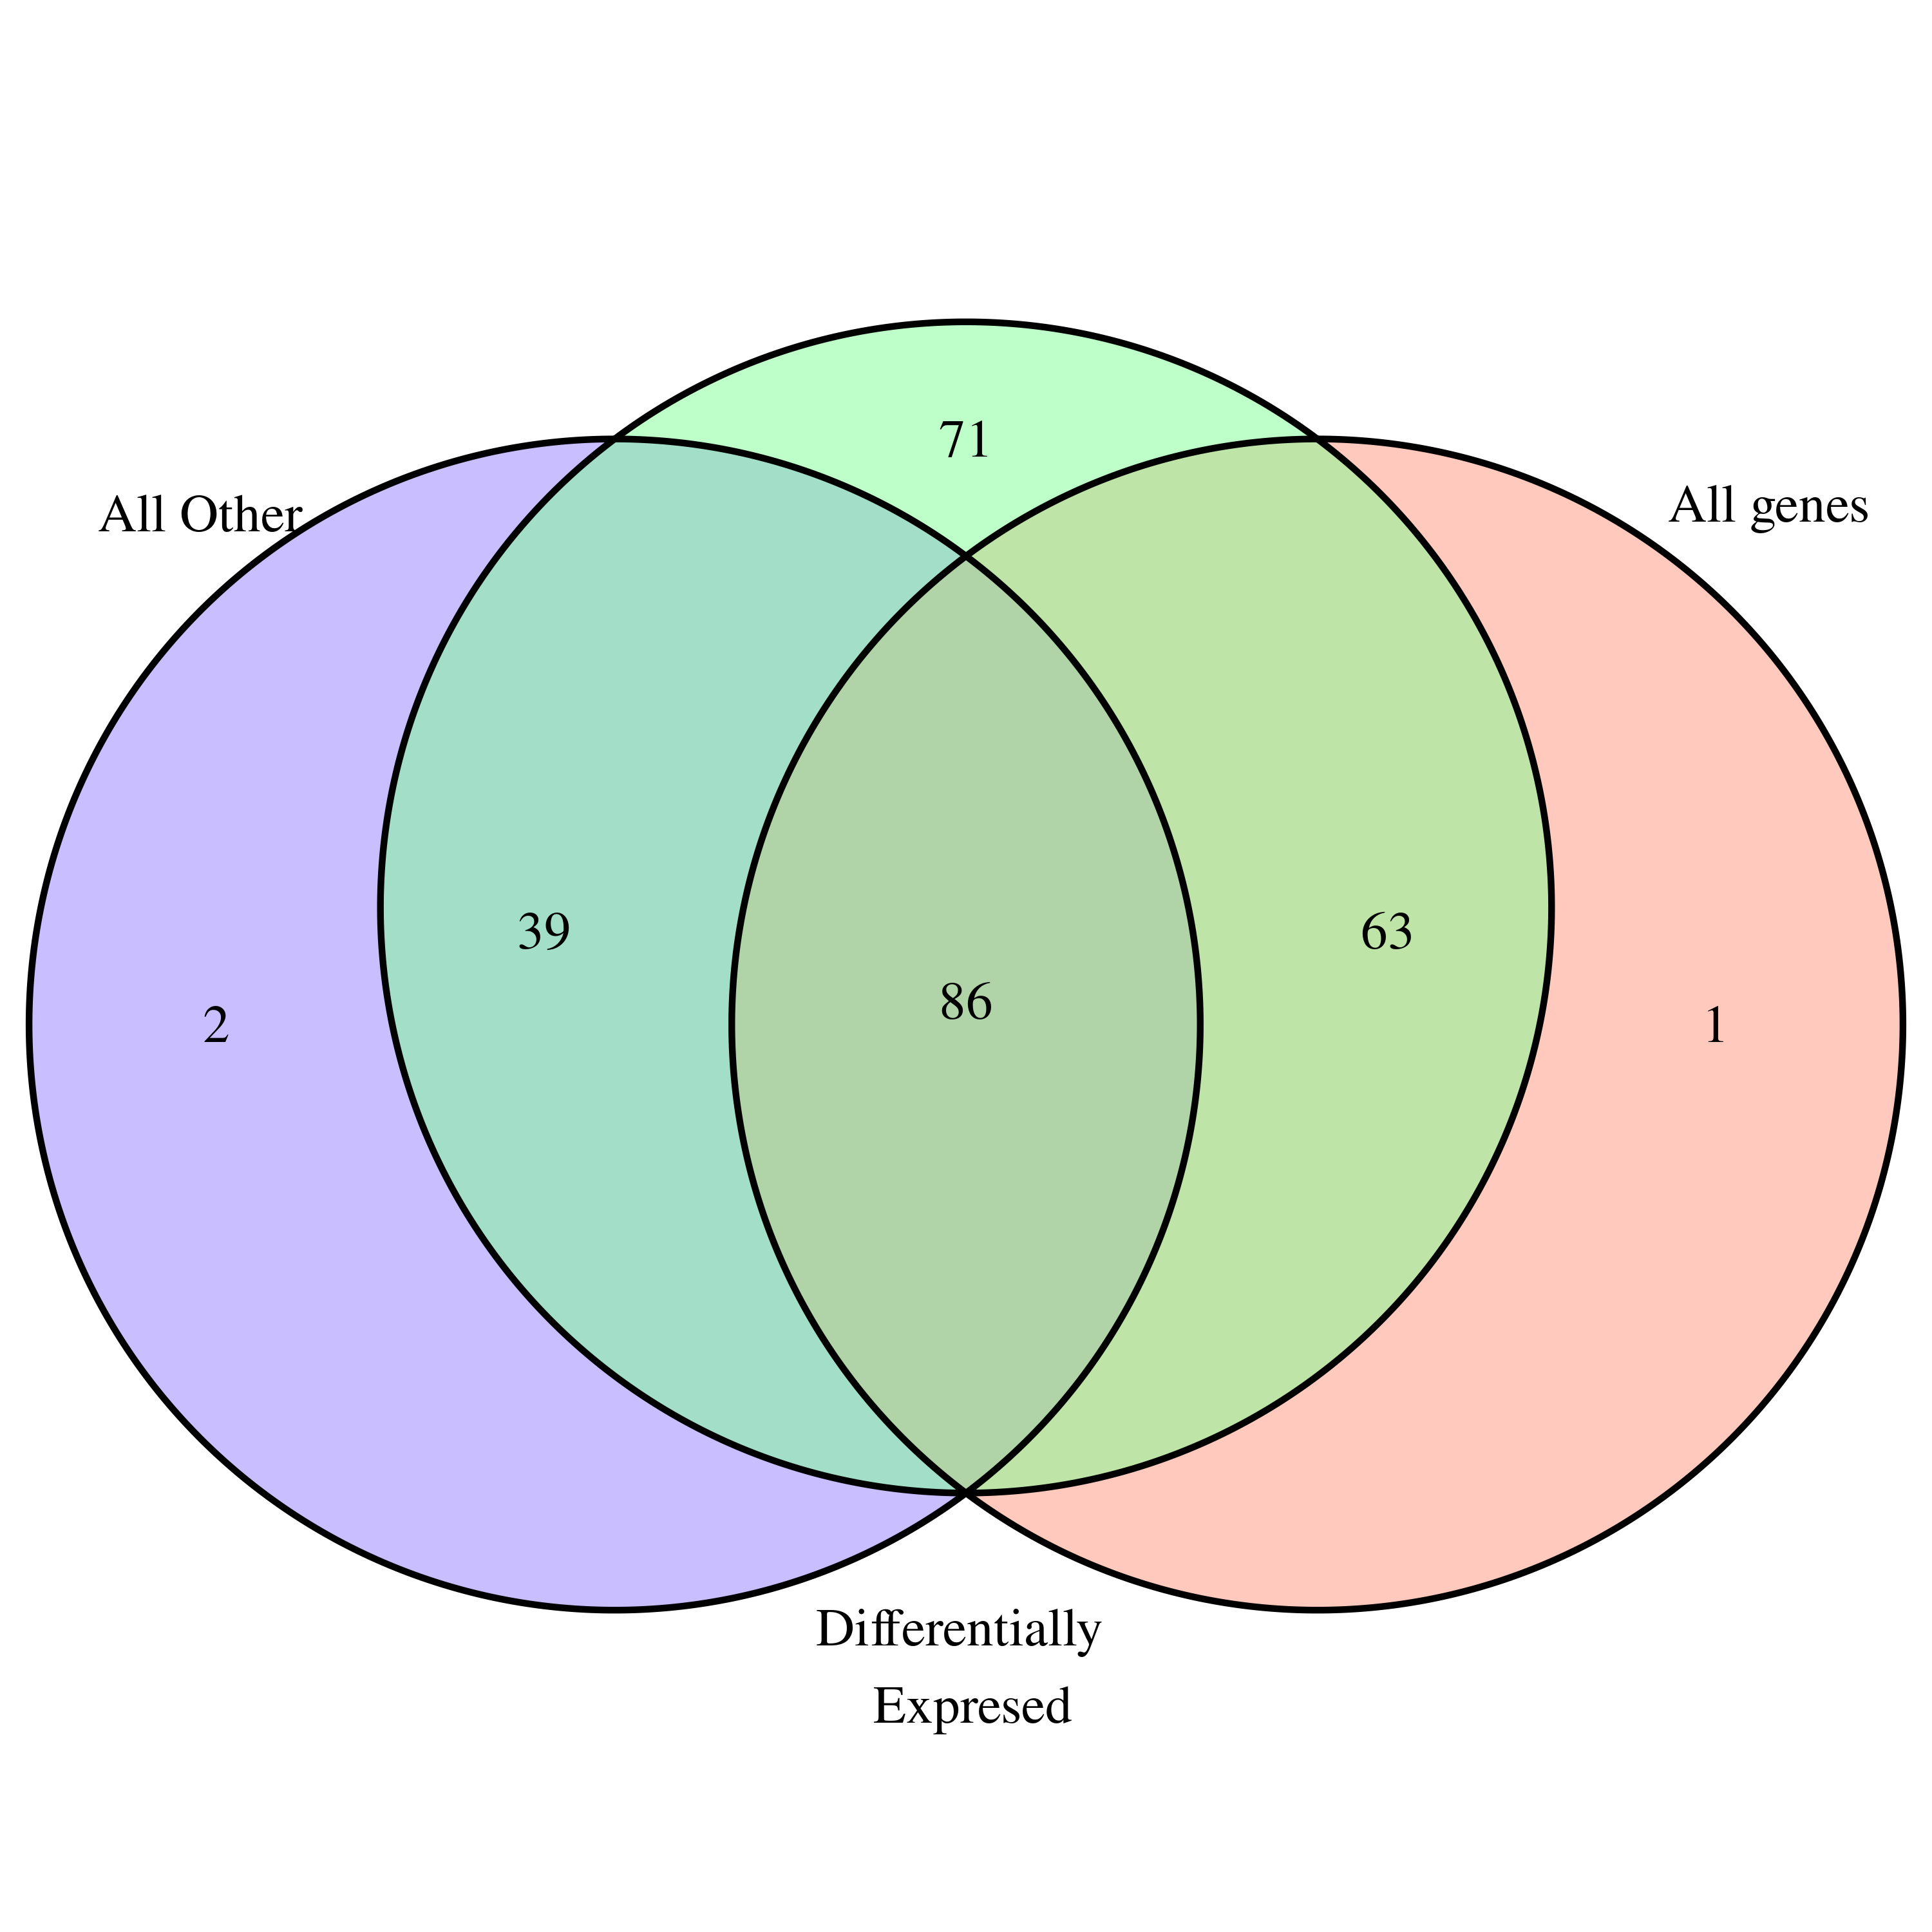
\includegraphics[width=0.6\textwidth]{./output/venn.png}
\caption{Venn diagram of the number of features selected by each dataset partition}
\label{fig:venn}
\end{figure}
\vspace{2em}

It is clear that most genes that were found out to be important are independent of the dataset they are originated. However, a significant finding is about the $71$ k-mers that were only found on the differentially expressed genes dataset. These features are the features that the boruta model found out to be important, as shown in \autoref{fig:boruta} (b). A way to overcome this is to filter out the k-mers where they only have a count of one or one "vote" (picked by a single model as important). This can be then further restricted by increasing the number of "votes" necessary to be considered important. 

\cleardoublepage
% ------------------------------------------------------------------------------------------------------
\section{Discussion}
\label{sec:discussion}

In this dissertation project, a conclusion has been successfully reached as to what genes are expressed in a different condition, when the fungus \emph{C. neoformans} is cultivated in a variety of media and temperatures. In addition to that, after finding those differentially expressed genes, a robust way of performing feature selection on the k-mers that these genes have was presented. This is an important task, as reducing the dimensions of this dataset is tremendously important due to the great size of these datasets. The results and the methods used can then be further used to implement machine learning models to predict which genes will be expressed in a fungus without performing expensive lab experiments and time-consuming RNA-sequencing
.
However, there exist various caveats in the report that need to be discussed in order to be transparent. First of all, the method used to identify the differentially expressed genes could be further improved by performing Analysis of Variance (ANOVA). The limitation of the simple t-test is that it only tests one condition at a time. A more interesting research question is what genes are differentially expressed between all the conditions and the timestamps at once. This is precisely what ANOVA tests, and it could be an improvement on the methods used. 

A second important task to be discussed is the hardware limitations. The full dataset of all the genes with all the k-mers as features, as well as the conditions one-hot encoded, occupies 150MB of memory. This is not an exceptionally large file size; however, the methods used to analyse the dataset might end up needing a lot more space. For example, maybe various bootstraps of the file need to be created, or cross-validation needs to be performed. In all these cases, the hardware required to do this calculation was not available. As a solution, the file was sampled by only including $1000$ rows. This can potentially impact the results by random chance, as the limit of $1000$ rows, set by the hardware, does not inspire a lot of trust. However, this caveat can easily be fixed by running the experiment on a server. A second more difficult but more effective fix would be to rewrite the analysis in a more computationally efficient language such as \textsf{C / C++}, or \textsf{Julia}.

Lastly, a significant caveat is the fact that only the variable "estimated counts" was selected to represent gene expression in order to be able to work with the \textsf{DESeq2 R} library. The transcripts per million (TPM) were not used at all. It would be interesting to compare the final results that the given methods produce by using the estimated counts as the target variable, with TPM as the target variable. 

In conclusion, while the final results of this project show great potential and can be further checked, interpreted, and reproduced by field scientists to validate them, there are various caveats that need to be addressed. This will make the results highly robust and reliable.  

\clearpage
% % ------------------------------------------------------------------------------------------------------
\bibliographystyle{plain}
\bibliography{background.bib}
\clearpage
\end{document}